%% -*- coding:utf-8 -*-
\documentclass[10pt,pdf,hyperref={unicode}]{beamer}
\input ./preamble.tex
\usetheme{Warsaw}
\title[Cryptography and quantum computations]{Classical
  cryptography\\Quantum computations}
\author{Ivan Murashko}
%\institute{Санкт Петербургский Государственный Политехнический Университет}
\date{}
\begin{document}

\begin{frame}
\titlepage
\end{frame}


\section{Introduction}

\begin{frame}{Introduction}
\begin{itemize}
\item Quantum mechanics
\item Quantum computations
\item Symmetric cryptography. Grover search algorithm (GSA)
\item Non-symmetric cryptography (RSA, Diffie-Hellman, Elliptic
curve) and Shor's algrorithm.
\end{itemize}
\end{frame}

\section{Quantum mechanics}
\begin{frame}{Two-level atom}
\begin{figure}
\centering

\input ../add/quant/picmeasurex.tex

\caption{Energy measurement for two-level atom. The atom is in pure
  state:  $\left|\psi\right> = 
  \frac{1}{\sqrt{2}}\left|a\right> + \frac{1}{\sqrt{2}}\left|b\right>$.
  Device can get either $E_a$ or $E_b$.
}
\label{fig:add:mesure_ex}
\end{figure}
\end{frame}

\begin{frame}{Two-level atom. $E_a$ measurement}
\begin{figure}
\centering

\input ../add/quant/picmeasurex_a.tex

\caption{Energy measurement for two-level atom. The atom is in pure
  state: $\left|\psi\right> = 
  \frac{1}{\sqrt{2}}\left|a\right> + \frac{1}{\sqrt{2}}\left|b\right>$.
  Device got $E_a$. The following wave function collapse occurs as a
  result of the measurement $\left|\psi\right> \to \left|a\right>$
}
\label{fig:add:mesure_ex_a}
\end{figure}
\end{frame}

\begin{frame}{Two-level atom. $E_b$ measurement}
\begin{figure}
\centering

\input ../add/quant/picmeasurex_b.tex

\caption{Energy measurement for two-level atom. The atom is in pure
  state: $\left|\psi\right> = 
\frac{1}{\sqrt{2}}\left|a\right> + \frac{1}{\sqrt{2}}\left|b\right>$.
Device got $E_b$. The following wave function collapse occurs as a
  result of the measurement $\left|\psi\right> \to \left|b\right>$
}
\label{fig:add:mesure_ex_b}
\end{figure}
\end{frame}

\begin{frame}{Schrödinger's cat}
 \begin{figure} 
   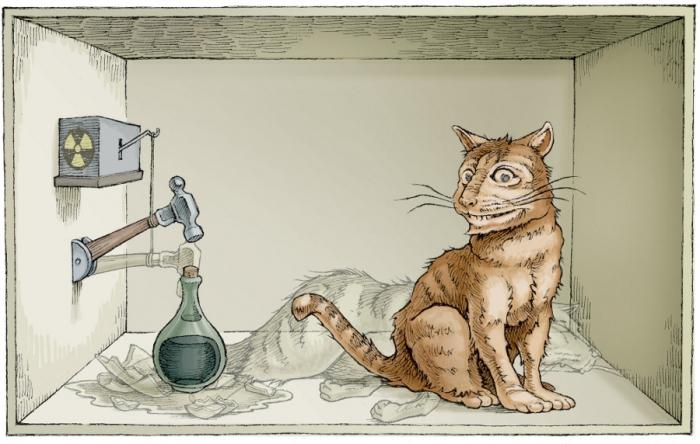
\includegraphics[width=100mm,scale=0.5]{catshred.jpg}
  \end{figure}
\end{frame}

\begin{frame}{Эксперимент Белла. Классический случай}
\[
f = \frac{1}{2}\left(
a b + a' b + a b' - a' b'
\right), a,a',b,b' \in \{-1, +1\}.
\]
следовательно
\(
f \in \{-1, +1\}
\)
и
\(
\left|\left<f\right>\right| \le 1
\)
\end{frame}

\begin{frame}{Эксперимент Белла. Квантовый случай}
\[
\left|\left<f\right>\right| = \sqrt{2} > 1
\]
\end{frame}


\begin{frame}{Отрицательные вероятности}
\[
\left<f\right> = \sum_{a,a',b,b'} p(a,a',b,b') f(a,a',b,b').
\]
следовательно для $\left|\left<f\right>\right| > 1$ необходимо
\[
\exists a,a',b,b': p(a,a',b,b') < 0
\]
\end{frame}

\section{Квантовые вычисления}
\begin{frame}{Классические вычисления}
\begin{figure}
\centering

\input ../part4/quantcomp/picclasscomp.tex

\caption{Классические вычисления. На вход подается число $x$ состоящее
  из $n$ бит, а на выходе имеем результат $y = f\left(x\right)$ описываемый $m$ битами}
\label{figQuantCompClassComp}
\end{figure}
\end{frame}

\begin{frame}{Квантовые вычисления}
\begin{figure}
\centering

\scalebox{.8}{\input{../part4/quantcomp/picquantcomp.tex}}

\caption{Квантовые обратимые вычисления. На вход подается число
  $\left|x\right>$ состоящее из $n$ кубит и затравка из нулевых
  состояний ($m$ кубит), а на выходе имеем результат $\left|y\right> =
  \left|f\left(x\right)\right>$ описываемый $m$ кубитами и исходное
  состояние $\left|x\right>$} 
\label{figQuantCompQuantComp}
\end{figure}
\end{frame}


\begin{frame}{Квантовые вычисления}
Классический случай
\[
x \to f(x)
\]
Квантовый случай
\begin{eqnarray}
\left|0\right>\left|0\right> + \left|1\right>\left|0\right> + \left|2\right>\left|0\right> +
\dots + \left|x\right>\left|0\right> + \dots \to
\nonumber \\
\to 
\left|0\right>\left|f(0)\right> + \left|1\right>\left|f(1)\right> + \left|2\right>\left|f(2)\right> +
\dots + \left|x\right>\left|f(x)\right> + \dots
\nonumber
\end{eqnarray}
\end{frame}


\section{Алгоритм Гровера}
\begin{frame}{Задача о поиске иголки в стоге сена}
\begin{figure}
\centering

\input ../part4/quantcomp/picsearch.tex

\caption{Поиск в неструктурированном объеме данных (поиск "иголки в
  стоге сена"). Классическая сложность $O(N)$}
\label{figQuantCompSearch}
\end{figure}
\end{frame}

\begin{frame}{Алгоритм Гровера. Схема}
\begin{figure}
\centering

\scalebox{1.0}{\input{../part4/quantcomp/picgrover.tex}}

\caption{Алгоритм Гровера. Сложность $ O(\sqrt{N})$}
\label{figQuantCompGrover}
\end{figure}
\end{frame}

\begin{frame}{Алгоритм Гровера. Схема повторяющегося элемента}
\begin{figure}
\centering

\scalebox{1.0}{\input{../part4/quantcomp/picgroverbase.tex}}

\caption{Алгоритм Гровера. Повторяющийся элемент}
\label{figQuantCompGrover}
\end{figure}
\end{frame}


\begin{frame}{Алгоритм Гровера. Принцип работы}
\begin{figure}
\centering

\scalebox{.9}{\input{../part4/quantcomp/picgroverinv.tex}}

\caption{Алгоритм Гровера. Инверсия фазы}
\label{figQuantCompGroverInv}
\end{figure}
\end{frame}

\begin{frame}{Алгоритм Гровера. Принцип работы}
\begin{figure}
\centering

\scalebox{.8}{\input{../part4/quantcomp/picgroverinvmiddle.tex}}

\caption{Алгоритм Гровера. Обращение относительно
  среднего.}
\label{figQuantCompGroverInvMiddle}
\end{figure}

\end{frame}


\begin{frame}{Влияние на рекомендации к использованию}
$O(N) \rightarrow O(\sqrt{N})$
ведет например к следующей рекомендации
$AES_{128} \rightarrow AES_{256}$
\end{frame}


\section{Алгоритм Шора}
\begin{frame}{Несимметричное шифрование}
\begin{itemize}
\item RSA и задача факторизации чисел
\item Diffie-Hellman и дискретный логарифм
\item Elliptic curve и дискретный логарифм
\end{itemize}
\end{frame}

\begin{frame}{RSA и задача о нахождении периода функций}
\[
N = p \cdot q
\]
\[
f\left(x, a\right) = a^x \mod N.
\]
Период функции $T = 2r$, т.е.
\begin{eqnarray}
a^{x+2r} \mod N = a^x \mod N,
\nonumber \\
a^{2r} \equiv 1 \mod N,
\nonumber \\
(a^r + 1)(a^r - 1)  \equiv 0 \mod N
\nonumber
\end{eqnarray}
\end{frame}

\begin{frame}{Алгоритм Шора}
\begin{figure}
\centering

\scalebox{.8}{\input{../part4/quantcomp/picquantperiodfinding.tex}}

\caption{ Определение периода функций с помощью квантового
  преобразования Фурье}
\end{figure}
\end{frame}


\begin{frame}{Алгоритм Шора. Нахождение периода функции 
  $f\left(x, a\right) = a^x \mod{N}$}
\begin{figure}
\centering

\scalebox{.65}{\input{../part4/quantcomp/picshorquantfourier1.tex}}

\caption{Алгоритм Шора. Нахождение периода функции 
  $f\left(x, a\right) = a^x \mod{N}$ при $a=2$, $N = 21$.}
\end{figure}
\end{frame}

\begin{frame}{Алгоритм Шора. Нахождение периода функции 
  $f\left(x, a\right) = a^x \mod{N}$}
\begin{figure}
\centering

\scalebox{.65}{\input{../part4/quantcomp/picshorquantfourier2.tex}}

\caption{Алгоритм Шора. Нахождение периода функции 
  $f\left(x, a\right) = a^x \mod{N}$ при $a=2$,  
  Значение функции 1 повторяется с периодом $r=6$.}
\end{figure}
\end{frame}

\begin{frame}{Алгоритм Шора. Нахождение периода функции 
  $f\left(x, a\right) = a^x \mod{N}$}
\begin{figure}
\centering

\scalebox{.6}{\input{../part4/quantcomp/picshorquantfourier3.tex}}

\caption{Алгоритм Шора. Нахождение периода функции 
  $f\left(x, a\right) = a^x \mod{N}$ при $a=2$. 
  Локальные максимумы преобразования Фурье 
  идут с периодом $\frac{M}{r} \approx 10.67$ ($M = 64$ - число отсчетов
  для преобразования Фурье)}
\end{figure}
\end{frame}

\begin{frame}{Рекомендованные значения для длины ключа}
 \begin{figure} 
   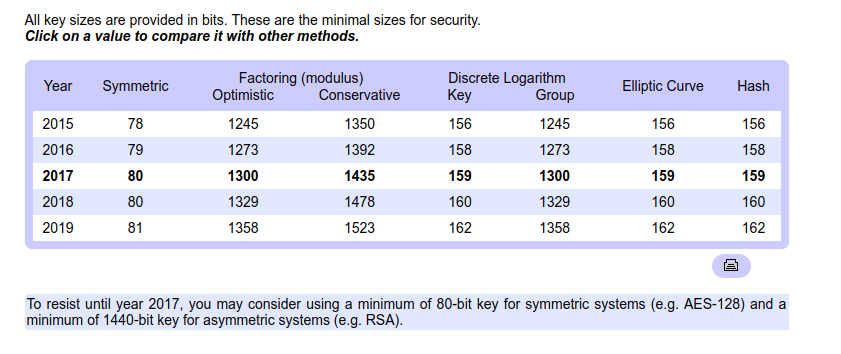
\includegraphics[width=120mm,scale=0.5]{keylengthcom.png}
  \end{figure}
\end{frame}

\begin{frame}{Влияние на рекомендации к использованию}
\begin{itemize}
\item RSA: 4096
\item DH: 2048/256
\item Elliptic curve: 512/256 (bitcoin) 
\end{itemize}

NSA не рекомендует использование алгоритмов на элиптических кривых для
внутреннего использования.
\end{frame}

\section{Заключение}
\begin{frame}{Что дальше?}
\begin{itemize}
\item Линейная алгебра (Матрицы)
\item Дискретная математика (Операции с остатком)
\end{itemize}
\end{frame}

\begin{frame}{Что дальше?}
https://github.com/ivanmurashko/lectures/tree/master/pdfs
 \begin{figure} 
   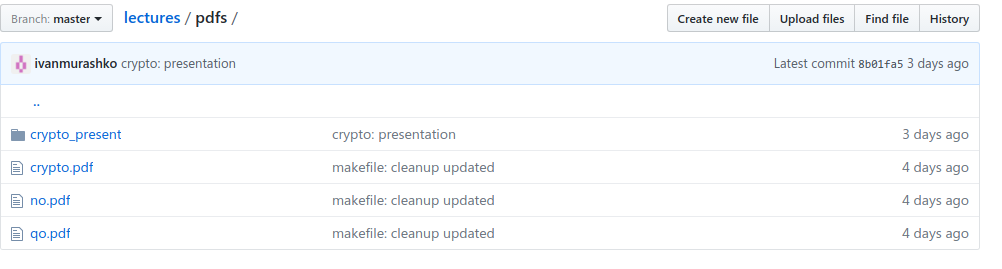
\includegraphics[width=90mm,scale=0.5]{github.png}
  \end{figure}
\end{frame}

\begin{frame}{Вопросы}
 \begin{figure} 
   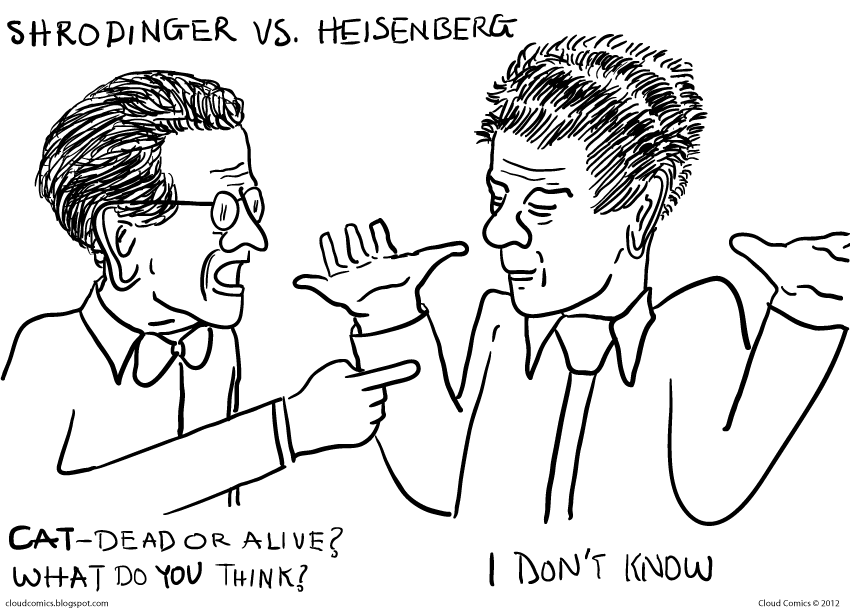
\includegraphics[width=90mm,scale=0.5]{questions.png}
  \end{figure}
\end{frame}

\end{document}
